% 本章按原 Word 结构转换。\templatehint 为写作提示，可用文档类 final 选项隐藏。

\chapter{需求分析与概要设计}\label{chap:3}
\smalltemplatehints

\templateblank

\section{系统需求分析}

\templatehint{目标：\hspace{5.28bp}说清楚你要做一个什么样的系统，给谁用，用来干什么。}

\subsection{系统边界与角色定义}

\templatehint{\hspace*{10.56bp}\makebox[10.56bp][l]{·}\hspace{5.16bp}内容：\hspace{5.28bp}明确系统涉及哪些用户群体。}

\templatehint{\hspace*{10.56bp}\makebox[10.56bp][l]{·}\hspace{5.16bp}写法：\hspace{5.28bp}“本系统面向三类用户：前台普通游客、前台注册会员和后端管理员。”}

\templatehint{\hspace*{10.56bp}\makebox[10.56bp][l]{·}\hspace{5.16bp}图表辅助：\hspace{5.28bp}画出系统上下文图或简单的用例图，展示角色与系统的交互。}

\ifecjtuguide\vspace{19.5bp}\fi
\subsection{功能性需求}

\templatehint{\hspace*{10.56bp}\makebox[10.56bp][l]{·}\hspace{5.16bp}内容：\hspace{5.28bp}分模块、分角色详细描述系统必须具备的功能。}

\templatehint{\hspace*{10.56bp}\makebox[10.56bp][l]{·}\hspace{5.16bp}写法：\hspace{5.28bp}不要只罗列列表，建议采用\hspace{5.28bp}“用例描述”\hspace{5.28bp}的方式。}

\templatehint{\hspace*{31.556bp}模块一：用户管理模块}

\templatehint{\hspace*{31.556bp}\makebox[10.56bp][l]{·}\hspace{5.16bp}用例UC-01：用户注册：用户通过手机号和验证码完成注册……}

\templatehint{\hspace*{31.556bp}\makebox[10.56bp][l]{·}\hspace{5.16bp}用例UC-02：用户登录：……}

\templatehint{\hspace*{31.556bp}模块二：核心业务模块}

\templatehint{\hspace*{36.836bp}\makebox[10.56bp][l]{·}\hspace{4.44bp}图表辅助：\hspace{4.56bp}用例图是标配，\hspace{-0.72bp}配合详细的用例规约表\hspace{-0.84bp}（包含：\hspace{-0.72bp}用例名称、\hspace{-0.78bp}参与者、\hspace{-0.78bp}前置条件、\\基本流程、后置条件）。}

\ifecjtuguide\vspace{19.5bp}\fi
\subsection{非功能性需求}

\templatehint{\hspace*{10.56bp}\makebox[10.56bp][l]{·}\hspace{5.16bp}内容：\hspace{5.28bp}系统的质量属性（体现你的工程素养）。}

\templatehint{\hspace*{10.56bp}\makebox[10.56bp][l]{·}\hspace{5.16bp}例子：}

\templatehint{\hspace*{21.12bp}\makebox[10.56bp][l]{·}\hspace{5.16bp}性能要求：\hspace{5.28bp}并发用户数、页面响应时间（如：小于3秒）。}

\templatehint{\hspace*{21.12bp}\makebox[10.56bp][l]{·}\hspace{5.16bp}安全性：\hspace{5.28bp}用户密码加密存储、数据传输加密、SQL注入防护。}

\templatehint{\hspace*{21.12bp}\makebox[10.56bp][l]{·}\hspace{5.16bp}可靠性：\hspace{5.28bp}系统7*24小时运行，重要数据备份策略。}

\templatehint{\hspace*{21bp}\makebox[10.56bp][l]{·}\hspace{5.16bp}易用性：\hspace{5.28bp}界面简洁，操作符合用户习惯。}

\ifecjtuguide\vspace{19.5bp}\fi
\section{系统概要设计}

\templateblank

\ifecjtuguide\vspace{19.5bp}\fi
\subsection{系统总体架构设计}

\templatehint{\hspace*{10.56bp}\makebox[10.56bp][l]{·}\hspace{5.16bp}内容：\hspace{5.28bp}描述系统的技术栈和分层结构。}

\templatehint{\hspace*{10.56bp}\makebox[10.56bp][l]{·}\hspace{5.16bp}写法：\hspace{5.28bp}如果是Web项目，通常是B/S架构，采用前后端分离。}

\templatehint{\hspace*{10.56bp}\makebox[10.56bp][l]{·}\hspace{5.16bp}图表辅助：\hspace{5.28bp}绘制系统架构图。}

\templatehint{\hspace*{21.12bp}\makebox[10.56bp][l]{·}\hspace{5.16bp}前端层：\hspace{5.28bp}Vue/React/小程序，负责界面展示。}

\templatehint{\hspace*{21.12bp}\makebox[10.56bp][l]{·}\hspace{5.16bp}后端层：\hspace{5.28bp}Spring~Boot/Django等，负责业务逻辑处理。}

\templatehint{\hspace*{21.12bp}\makebox[10.56bp][l]{·}\hspace{5.16bp}数据层：\hspace{5.28bp}MySQL/Redis，负责数据存储。}

\templatehint{\hspace*{21.12bp}\makebox[10.56bp][l]{·}\hspace{5.16bp}基础设施层：\hspace{5.28bp}服务器、对象存储等。}

\templatehint{\hspace*{10.56bp}\makebox[10.56bp][l]{·}\hspace{5.16bp}注意：\hspace{5.28bp}要解释为什么选这个架构（如：为了高并发、为了可维护性）。}

\ifecjtuguide\vspace{19.5bp}\fi
\subsection{系统功能模块划分}

\templatehint{\hspace*{10.56bp}\makebox[10.56bp][l]{·}\hspace{5.16bp}内容：\hspace{5.28bp}将3.1节的需求映射成具体的软件模块。}

\templatehint{\hspace*{10.56bp}\makebox[10.56bp][l]{·}\hspace{5.16bp}写法：\hspace{5.28bp}将系统拆分成多个子系统或模块，并说明模块间的调用关系。}

\templatehint{\hspace*{10.56bp}\makebox[10.56bp][l]{·}\hspace{3.96bp}图表辅助：\hspace{5.28bp}绘制功能模块图（分层结构图）。例如：顶层是“在线考试系统”，第二层是“用户端”和“管理端”，第三层再细分。}

\ifecjtuguide\vspace{19.5bp}\fi
\subsection{系统业务流程设计}

\templatehint{\hspace*{10.56bp}\makebox[10.56bp][l]{·}\hspace{5.16bp}内容：\hspace{5.28bp}选取核心业务逻辑，描述数据流转过程。}

\templatehint{\hspace*{10.56bp}\makebox[10.56bp][l]{·}\hspace{3.84bp}图表辅助：\hspace{5.28bp}绘制业务流程图或活动图。例如：“用户下单”的流程：发起支付\hspace{5.28bp}->\hspace{5.28bp}检查库存\hspace{5.28bp}->\hspace{5.28bp}扣减余额\hspace{5.28bp}->\hspace{5.28bp}生成订单。}

\subsection{数据库概念结构设计}

\templatehint{\hspace*{15.84bp}\makebox[10.56bp][l]{{\color{black}·}}\hspace{5.16bp}内容：数据库相关技术架构的概述，具体设计详见第4章。}

\subsection{系统接口设计（可选，但建议写）}

\templatehint{\hspace*{10.56bp}\makebox[10.56bp][l]{·}\hspace{5.16bp}内容：\hspace{5.28bp}如果是前后端分离或涉及第三方系统，列出核心API的设计风格。}

\templatehint{\hspace*{10.56bp}\makebox[10.56bp][l]{·}\hspace{5.16bp}写法：\hspace{5.28bp}RESTful风格，简要描述几个核心接口的URL、请求方式、参数和返回值示例。}

\subsection{界面原型设计}

\templatehint{\hspace*{10.56bp}\makebox[10.56bp][l]{·}\hspace{5.16bp}内容：\hspace{5.28bp}展示几张核心界面的低保真或高保真原型图。}

\templatehint{\hspace*{10.56bp}\makebox[10.56bp][l]{·}\hspace{5.16bp}说明：\hspace{5.28bp}简单解释一下界面的布局逻辑和用户操作路径。这能证明你在设计时考虑了用户体验。}

\ifecjtuguide\vspace{19.5bp}\fi
\templatehint{写作注意事项：}

\templatehint{1.\hspace{5.28bp}逻辑对应：\hspace{5.28bp}确保概要设计的内容完全覆盖了需求分析中提出的功能。不要让评委觉得“你分析了一堆需求，结果设计出来的模块对不上”。}

\templatehint{2.\hspace{5.28bp}图文并茂：\hspace{4.668bp}这一章最忌讳纯文字。\hspace{-0.48bp}一张好的架构图或E-R图，\hspace{-0.48bp}胜过几百字的描述。\hspace{-0.6bp}建议使用Visio、\\Draw.io或ProcessOn绘制。}

\templatehint{3.\hspace{5.28bp}避免过度细节：\hspace{5.28bp}这一章叫“概要设计”，不要在这里贴大段的HTML代码、SQL建表语句或具体的算法源码，那是“详细设计”或“系统实现”章的内容。}

\templatehint{4.\hspace{5.28bp}技术选型要有理由：\hspace{5.28bp}不要只是罗列用了Spring~Boot、MySQL，要简单说一句为什么（比如：因为Spring~Boot生态完善，便于快速开发；MySQL开源且满足数据一致性要求）。}

\templatehint{{\xeCJKsetup{CJKglue=\hskip0.014bp}5.\hspace{5.28bp}关注核心痛点：\hspace{5.28bp}如果你的毕业设计是做“基于深度学习的某某推荐系统”，那么在需求分析时要强\linebreak} 调“为什么需要推荐”，在概要设计时要画出“推荐服务的模块位置”和“数据流”。}

% 原 Word 的流程图作为图片保留其线型、填色和文字位置。
\clearpage
\begingroup\ecjtuwordgridfalse
\vspace*{-19.7545bp}
\begin{figure}[H]
\centering
\captionsetup{skip=4.1935bp}
\hspace*{-0.088bp}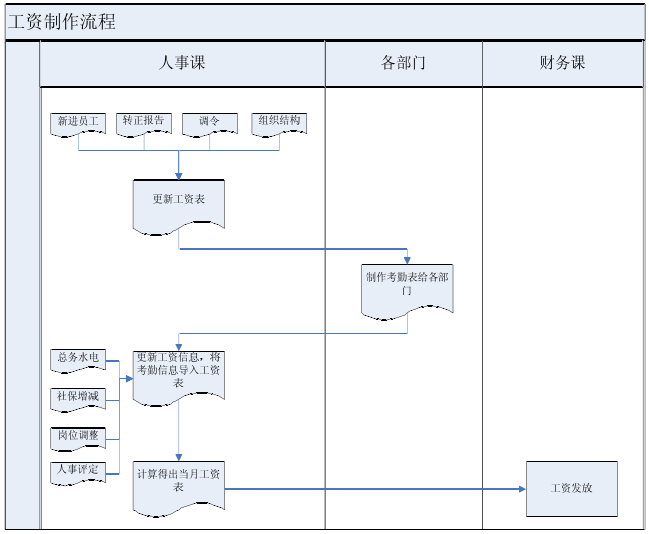
\includegraphics[width=369bp,height=303.6bp]{assets/salary-flow.png}
\caption{工资制作流程图}\label{fig:salary}
\end{figure}
\vspace{-17.43bp}
\normaltemplatehints
\templatehint{\xeCJKsetup{PunctStyle=quanjiao}\mbox{\xeCJKsetup{PunctStyle=plain}（}论文中\guidanceem{图}\hspace{6bp}的画法，注意以下几点：1\hspace{6bp}图要用word画，或者采用粘贴方式，不能使用截\linebreak
图方式，否则打印出来图的效果很不清晰。2\hspace{6bp}\guidanceem{图的标题}\hspace{6bp}要写在\guidanceem{图的下方}，\guidanceem{居中}，用\hspace{5.52bp}\guidanceem{5\hspace{5.52bp}号}\linebreak
\guidanceem{黑体字}。3\hspace{6bp}\guidanceem{图中的文字}采用\guidanceem{5号宋体字}。4\hspace{6bp}\guidanceem{每章}的所有图采用\guidanceem{顺序编号}，如图3-1，图3-2\linebreak
等）}

\vspace{11.71bp}
\begin{table}[H]
\captionsetup{skip=0.03bp}
\caption{工资管理问题点}\label{tab:salary}
\tablefont
\renewcommand{\arraystretch}{1}
\setlength{\tabcolsep}{5.16bp}
\setlength{\arrayrulewidth}{0.48bp}
\setbox\strutbox=\hbox{\ecjtuwordstrut{13.56}{6}}
\hspace*{21.36bp}\begin{tabular}{|p{48.596bp}|p{61.23bp}|p{132.74bp}|p{97.71bp}|}
\hline
涉及点 & 目前做法 & 存在问题 & 希望改善\\\hline
考勤 & 各部门汇总 & 考勤存在虚报、错误时无法核对，导致错误。 & 考勤准确\\\hline
工资计算 & 凭公式计算 & 灵活，\hspace{-4.68bp}但易出错，\hspace{-4.68bp}且不易检查。 & {\xeCJKsetup{CJKglue=\hskip0.36bp}固定某些必要内容，}\newline 使出错率降低。\\\hline
人员信息 & {\xeCJKsetup{CJKglue=\hskip2.1bp}以批注的形}\newline 式予以提醒 & 易出现遗漏现象，且人事系统与工资系统无法相对应。 & {\xeCJKsetup{CJKglue=\hskip0.33bp}\XeTeXcharclass"FF0C=1\relax 使用同一系统，达到}\newline 信息共享目的。\\\hline
\end{tabular}
\end{table}
\vspace{1.95bp}
\templatehint{\xeCJKsetup{PunctStyle=quanjiao}\mbox{\xeCJKsetup{PunctStyle=plain}（}论文中\guidanceem{表}\hspace{6bp}的画法，注意以下几点：1\hspace{6bp}表要用word画，不能使用截图方式，否则打印出\linebreak
来效果很不清晰。2\hspace{6bp}\guidanceem{表的标题}\hspace{6bp}要写在\guidanceem{表的上方}，\guidanceem{居中}，用\guidanceem{5号黑体字}。3\hspace{6bp}\guidanceem{表中的文字}\hspace{6bp}采\linebreak
用\guidanceem{5号宋体字}。4\hspace{6bp}\guidanceem{每章}\hspace{6bp}的所有表采用\hspace{6bp}\guidanceem{顺序编号}，如表3-1，表3-2等）}
\endgroup

\normaltemplatehints
